%%%%%%%%%%%%%%%%%%%%%%%%%%%%%%%%%%%%%%%%%
% Beamer Presentation
% LaTeX Template
%
% This template has been downloaded from:
% http://www.LaTeXTemplates.com
%
% This template has been altered after it was downloaded from the 
% above link
%
% License:
% CC BY-NC-SA 3.0 (http://creativecommons.org/licenses/by-nc-sa/3.0/)
%
%%%%%%%%%%%%%%%%%%%%%%%%%%%%%%%%%%%%%%%%%

%----------------------------------------------------------------------------------------
%	PACKAGES AND THEMES


\documentclass{beamer}

\mode<presentation> {

% The Beamer class comes with a number of default slide themes
% which change the colors and layouts of slides. Below this is a list
% of all the themes, uncomment each in turn to see what they look like.

%\usetheme{default}
%\usetheme{AnnArbor}
%\usetheme{Antibes}
%\usetheme{Bergen}
%\usetheme{Berkeley}
%\usetheme{Berlin}
%\usetheme{Boadilla}
%\usetheme{CambridgeUS}
%\usetheme{Copenhagen}
%\usetheme{Darmstadt}
%\usetheme{Dresden}
\usetheme{Frankfurt}
%\usetheme{Goettingen}
%\usetheme{Hannover}
%\usetheme{Ilmenau}
%\usetheme{JuanLesPins}
%\usetheme{Luebeck}
%\usetheme{Madrid}
%\usetheme{Malmoe}
%\usetheme{Marburg}
%\usetheme{Montpellier}
%\usetheme{PaloAlto}
%\usetheme{Pittsburgh}
%\usetheme{Rochester}
%\usetheme{Singapore}
%\usetheme{Szeged}
%\usetheme{Warsaw}

% As well as themes, the Beamer class has a number of color themes
% for any slide theme. Uncomment each of these in turn to see how it
% changes the colors of your current slide theme.

%\usecolortheme{albatross}
%\usecolortheme{beaver}
%\usecolortheme{beetle}
%\usecolortheme{crane}
%\usecolortheme{dolphin}
\usecolortheme{dove}
%\usecolortheme{fly}
%\usecolortheme{lily}
%\usecolortheme{orchid}
%\usecolortheme{rose}
%\usecolortheme{seagull}
%\usecolortheme{seahorse}
%\usecolortheme{whale}
%\usecolortheme{wolverine}

% Here is an overview of possible theme and colortheme combinations:
% https://hartwork.org/beamer-theme-matrix/

%\setbeamertemplate{footline} % To remove the footer line in all slides uncomment this line
%\setbeamertemplate{footline}[page number] % To replace the footer line in all slides with a simple slide count uncomment this line

%\setbeamertemplate{navigation symbols}{} % To remove the navigation symbols from the bottom of all slides uncomment this line
}

\usepackage{graphicx} % Allows including images
\usepackage{booktabs} % Allows the use of \toprule, \midrule and \bottomrule in tables
\usepackage{xcolor} % allows use of colors
\usepackage{appendixnumberbeamer} % Allows use of \appendix. Slides appearing after will not be part of the frame counter or navigation panel
\usepackage{todonotes} % Allows use of \missingfigure

% Following lines makes a section overview at the beginning of each section 
\setbeamertemplate{caption}{\raggedright\insertcaption\par}
\AtBeginSection[]
{
 \begin{frame}<beamer>
 \frametitle{Overview}
 \tableofcontents[currentsection]
 \end{frame}
}

% Define commands
\newcommand{\pd}[1]{\partial_{#1}}
\newcommand{\pdd}[1]{\partial_{#1}^2}

%----------------------------------------------------------------------------------------
%   TITLE PAGE
%----------------------------------------------------------------------------------------

\title[An idealized study of flow across submarine canyons]{An idealized study of flow across submarine canyons: \small Analytical and numerical approaches to canyon dynamics with applications to the LoVe ocean region} % The short title appears at the bottom of every slide (dependent on theme), the full title is only on the title page

\author{Anna Lina Petrusevi\v ci\=ut\.e Sjur\\
Supervisor: Pål Erik Isachsen} % Your name
\institute[UiO] % Your institution as it will appear on every slide (dependent on theme), may be shorthand to save space
{
University of Oslo \\ % Your institution for the title page
\medskip
%\textit{kari@mail.uio.no} % Your email address
}
\date{August 19, 2021} % Date, can be changed to a custom date

\begin{document}

{
%\usebackgroundtemplate{\includegraphics[width=\paperwidth]{figures/dybdedata_stor.pdf}} % background of first slide
\begin{frame}
\titlepage % Print the title page as the first slide
\end{frame}
}

%\begin{frame}
%\frametitle{Overview} % Table of contents slide, comment this block out to remove it
%\tableofcontents % Throughout your presentation, if you choose to use \section{} and \subsection{} commands, these will automatically be printed on this slide as an overview of your presentation
%\end{frame}

%----------------------------------------------------------------------------------------
%   PRESENTATION SLIDES
%----------------------------------------------------------------------------------------

%------------------------------------------------
\section{Introduction} % Sections can be created in order to organize your presentation into discrete blocks, all sections and subsections are automatically printed in the table of contents as an overview of the talk
%------------------------------------------------

\subsection{Motivation} % A subsection can be created just before a set of slides with a common theme to further break down your presentation into chunks
\begin{frame}{Sightings of sperm whales in Norwegian and adjacent waters}
    \begin{figure}
    \centering
    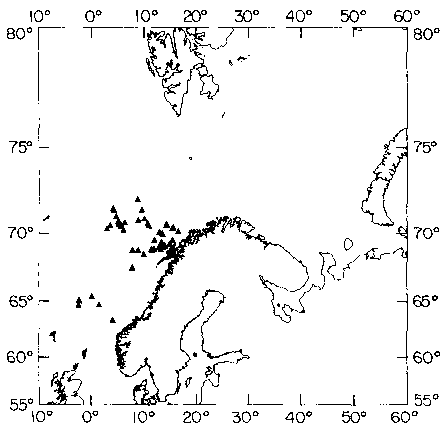
\includegraphics[width = 0.5\textwidth]{figures/whalesitings_large.pdf}
    %\missingfigure{Insert map of LoVe bathymtry here.}
    \caption{Figure from Christensen, 1992.} %\cite{CianoJ.N2001POSW}}
\end{figure}
\end{frame}

\begin{frame}{The Lofoten-Vesterålen ocean region}
\begin{figure}
    \centering
    \includegraphics[width=\linewidth]{figures/dybdedata_stor.pdf}
\end{figure}
\end{frame}

\begin{frame}{Canyon dynamics}
\begin{columns}
\column{0.65\linewidth}
\begin{itemize}
   % \item Submarine canyons are steep-sided valleys cut into the seabed of a continental slope.
    \item There is an \textbf{asymmetrical response} to along-shore flow in opposite directions. 
    \item When the flow is \textbf{retrograde}, submarine canyons significantly alter the flow.
    \item For \textbf{prograde} flow, the response is much weaker.
    \item Zhang and Lentz (2017) suggests this behaviour is due to arrested topographic waves.
    \item Related problem: Atmospheric mountain-waves. 
    \item Currents in LoVe are prograde. 
\end{itemize}
\column{0.35\linewidth}
\begin{figure}
    \centering
    %\missingfigure{Insert a picture of submarine canyon here.}
    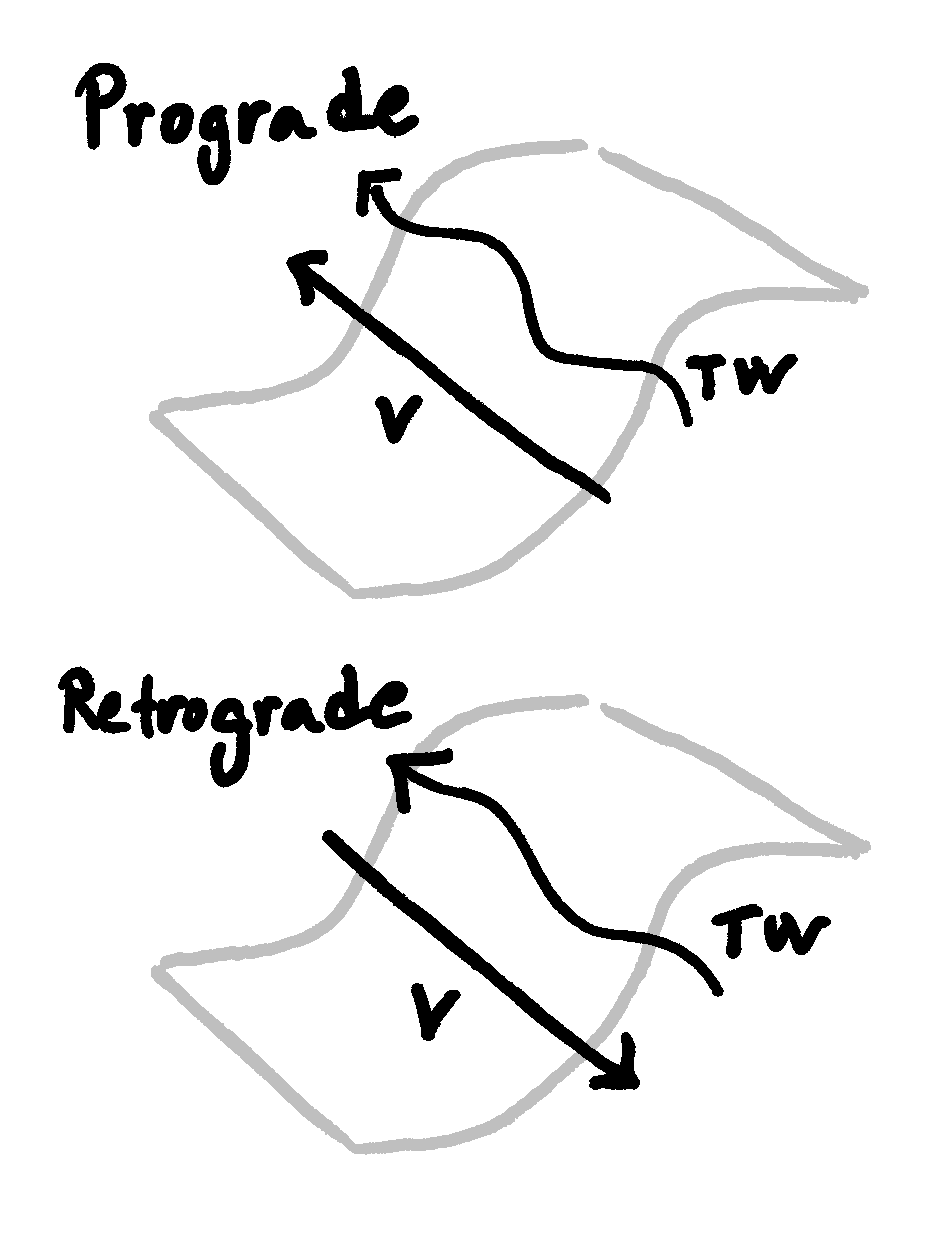
\includegraphics[width=\linewidth]{figures/prograde_retrograde_sketch.pdf}
\end{figure}
\end{columns}
\end{frame}

%\begin{frame}{Bleik Canyon showing 180 documented sightings of sperm whales}
%    \begin{figure}
%    \centering
%    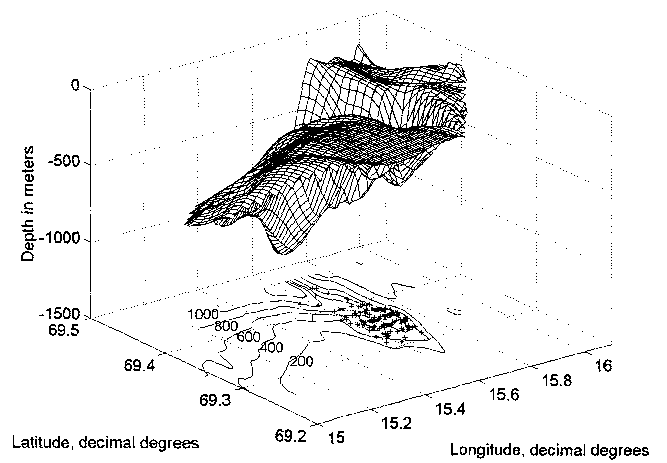
\includegraphics[width = 0.8\textwidth]{figures/whalesitings_bleikdjupet.pdf}
    %\missingfigure{Insert map of LoVe bathymtry here.}
%    \caption{Figure from Ciano and Huele, 2001.} %\cite{CianoJ.N2001POSW}}
%\end{figure}
%\end{frame}

\subsection{Research questions}

\begin{frame}{Research questions}
    \begin{itemize}
    \item Can quasi-geostrophic theory be used to describe flow patterns over a submarine canyon?
    \item Does a canyon affect the cross-slope exchange in a highly turbulent field?
    \item \textcolor{black}{What is the effect of periods of reversed wind on the cross-slope exchange under mean prograde flow over a canyon?} 
\end{itemize}

\end{frame}

%\subsection{Methods}
%\begin{frame}{Methods}
%    \begin{columns}
%\column{0.65\linewidth}

%\begin{itemize}
%    \item Use quasi-geostrophy to describe arrested topographic waves
%    \begin{itemize}
%        \item Compare theoretical response with numerical model runs
%    \end{itemize}
%    \item Run simulations of wind-forced flow over a canyon using ROMS
%    \begin{itemize}
%        \item Let run for longer period
%        \item Reverse wind for a short period
%    \end{itemize}
%    \item Cross-slope water exchange was approximated by computing the cross-slope transport of a passive tracer. 
%\end{itemize}
%\column{0.35\linewidth}
%\begin{figure}
%    \centering
%    
\includegraphics[width=0.9\linewidth]{figures/ROMS_logo.png}
%\end{figure}
%\end{columns}
%\end{frame}

\section{Analytical model}

\begin{frame}{Assumptions}
\begin{columns}
\column{0.5\linewidth}
\textbf{Barotropic}
\begin{figure}
    %\centering
    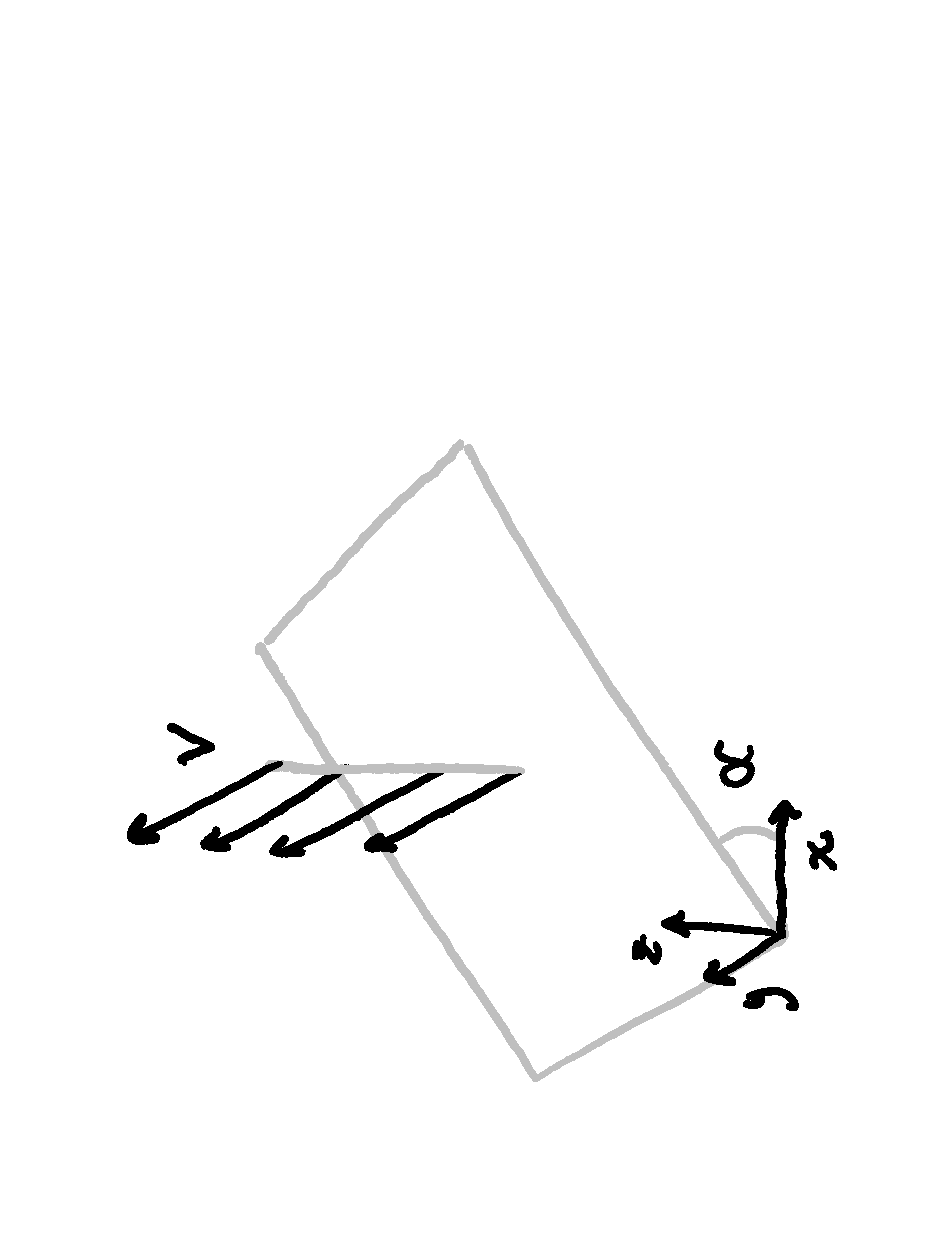
\includegraphics[trim=1cm 0 0 7cm,clip,angle=-90,origin=c,width=0.6\linewidth]
    {figures/barotropic_parameterss.pdf}
\end{figure}
\column{0.5\linewidth}
\textbf{Baroclinic}
\begin{figure}
    %\centering
    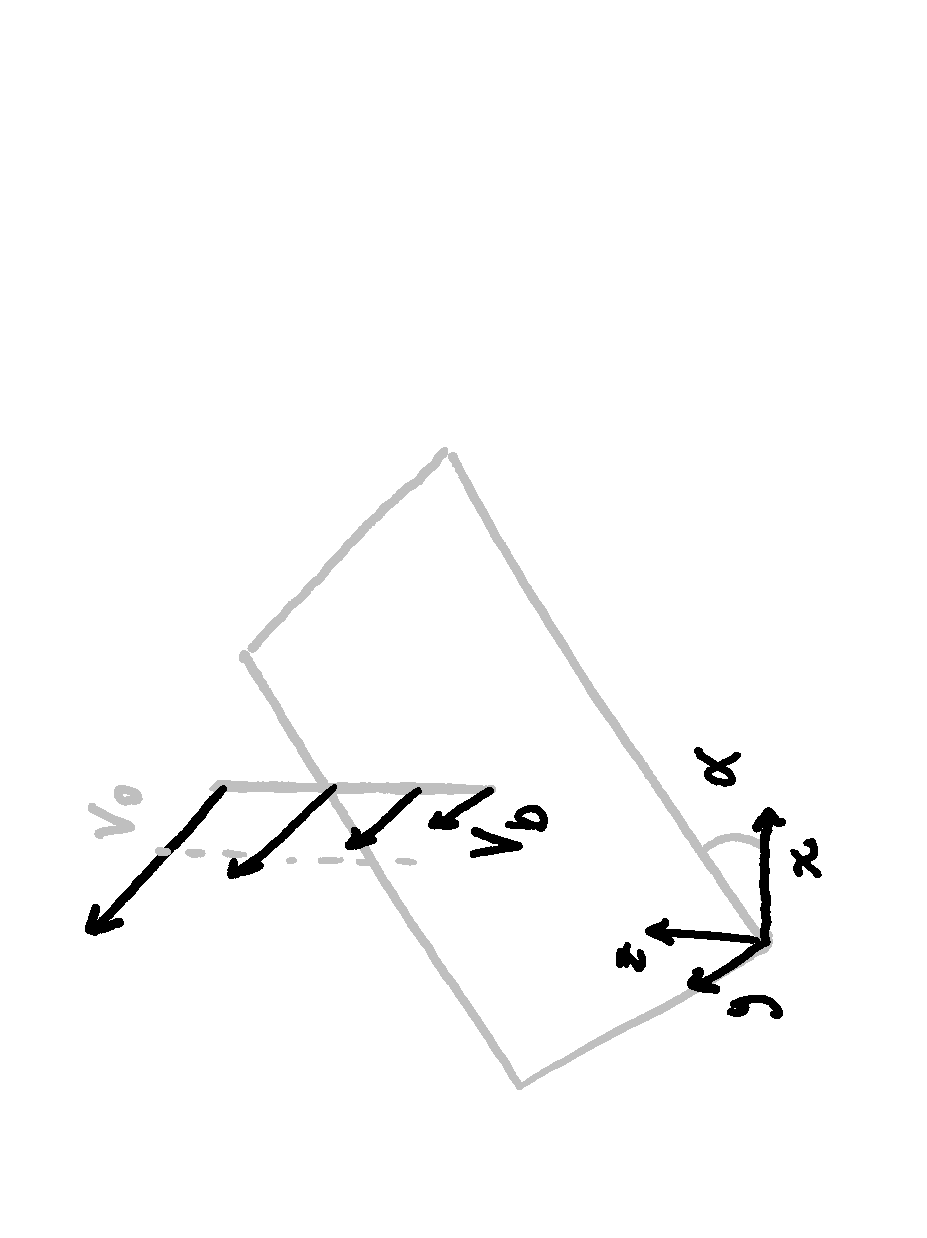
\includegraphics[trim=1cm 0 0 7cm,clip,angle=-90,origin=c,width=0.6\linewidth]{figures/baroclinic_parameterss.pdf}
\end{figure}

\end{columns}
Use the quasi-geostrophic potential vorticity equations + boundary equations.

Assume a streamfunction solution on the form
\begin{equation*}
    \psi = \operatorname{Re}\left[\sum_{k,l} \hat{\psi}_{k,l}e^{ikx+ily}\right], \qquad \kappa^2 = k^2+l^2 
\end{equation*}

\end{frame}

\subsection{Barotropic unstratified flow}
\begin{frame}{Barotropic flow}

The Fourier coefficients of the streamfunction response can be written as
\begin{equation*}
    \hat{\psi}_{k,l} = \frac{ \hat{h}_{k,l}\frac{f_0}{h_0}}{\left( \kappa^2 + \frac{\alpha f_0}{h_0V} + \frac{\pdd{x}V}{V} - i \frac{r\kappa^2}{Vl}\right)}
\end{equation*}
\begin{columns}
\column{0.5\linewidth}
Wavenumber of barotropic arrested wave:
\begin{equation*}
    \kappa_{s}^2 = - \frac{\alpha f_0}{h_0V} - \frac{\pdd{x}V}{V} 
\end{equation*}

\begin{equation*}
    \hat{\psi}_{k,l} = \frac{\hat{h}_{k,l}\frac{f_0}{h_0}}{\left( \kappa^2 - \kappa_{s}^2 - i \frac{r\kappa^2}{Vl}\right)}
\end{equation*}
\column{0.5\linewidth}
\begin{figure}
    \centering
    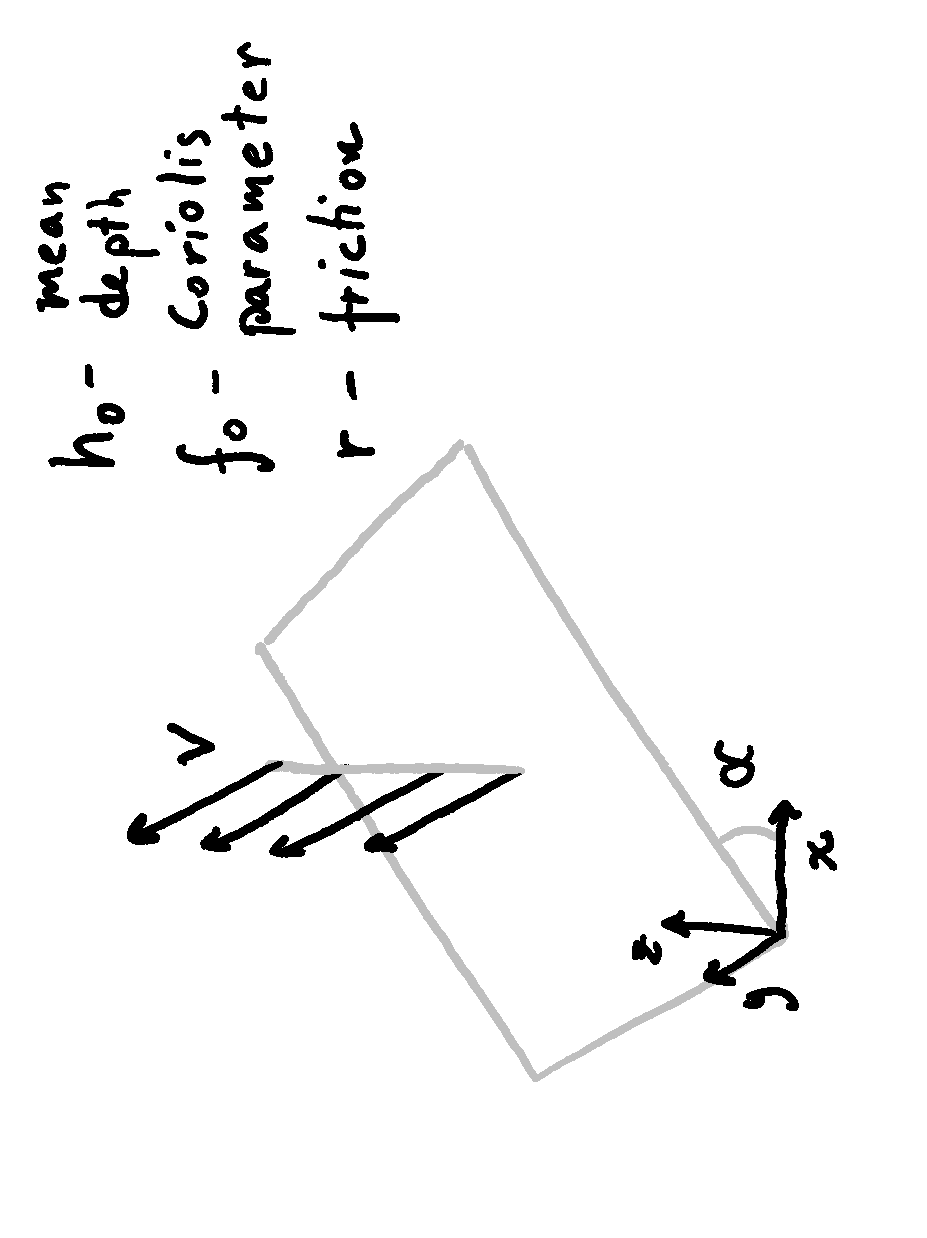
\includegraphics[angle=-90,origin=c,width=\linewidth]
    {figures/barotropic_parameters.pdf}
\end{figure}

\end{columns}
%Arrested wave number:
%\begin{equation*}
%    \kappa_{s,bt}^2 = -\left(\frac{\alpha f_0}{h_0V} + %\frac{\pdd{x}V}{V}\right)
%\end{equation*}
\end{frame}

\subsection{Baroclinic stratified flow}
%\begin{frame}{Baroclinic flow}
%\footnotesize
%\begin{multline*}
%    \hat{\psi}_{k,l}(z) = \hat{h}_{k,l}N\left(\left(\kappa^2 + \frac{\pdd{x}V}{V_0} \right)^{\frac{1}{2}} + \frac{f_0\pd{z}V}{NV_b} + \frac{\alpha N}{V_b} - i\frac{rN\kappa^2}{V_bl}\right)^{-1}e^{-\mu z},
%    \\ \mu = \frac{N}{|f_0|}\left( \kappa^2+\frac{\pdd{x}V_0}{V_0}\right)^{\frac{1}{2}} 
%\end{multline*}
%\normalsize
%\begin{columns}
%\column{0.5\linewidth}
%\begin{figure}
%    \centering
%    \includegraphics[angle=-90,origin=c,width=\linewidth]
%    {figures/baroclinic_parameters.pdf}
%\end{figure}
%\column{0.5\linewidth}
%Wavenumber of baroclinic arrested wave:
%\begin{equation*}
%    \kappa_{s,bc}^2 = \left(-\frac{f_0\pd{z}V}{NV_b} - \frac{\alpha N}{V_b}\right)^2 - \frac{\pdd{x}V}{V_0}
%\end{equation*}
%\begin{equation*}
%    \hat{\psi}_{k,l}(z) = \frac{\hat{h}_{k,l}N}{\left( \kappa - \kappa_{s,bc} - i \frac{rN\kappa^2}{V_bl}\right)}e^{-\mu z}
%\end{equation*}

%\end{columns}
%Arrested wave number:
%\begin{equation*}
%    \kappa_{s,bc}^2 = \left(-\frac{f_0\pd{z}V}{NV_b} - \frac{\alpha N}{V_b}\right)^2 - \frac{\pdd{x}V}{V_0}
%\end{equation*}

%\end{frame}

\begin{frame}
\frametitle{Amplitude spectrum}
\begin{figure}
\centering
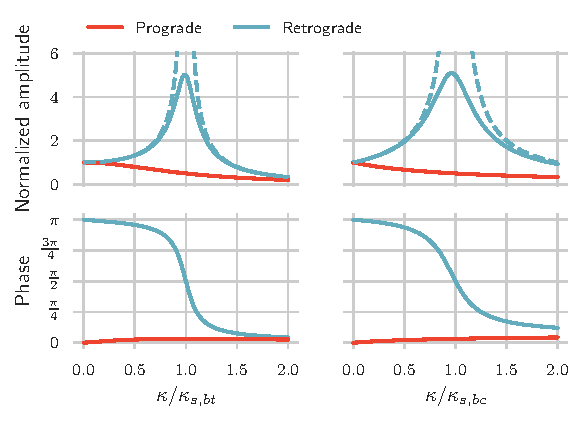
\includegraphics{figures/amplitude_phase.pdf}
\end{figure}
\end{frame}

\begin{frame}
\frametitle{Streamfunction response to a canyon}
\only<1>{
\begin{figure}
\centering
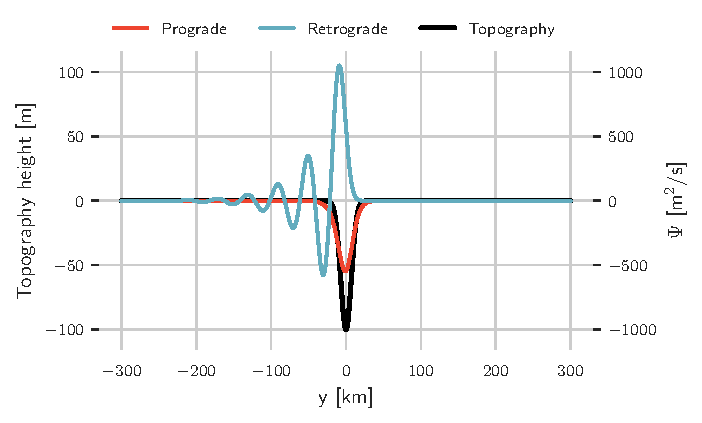
\includegraphics[width=\textwidth]{figures/unstratified_psi(y).pdf}
\end{figure}}

\only<2>{
\begin{figure}
\centering
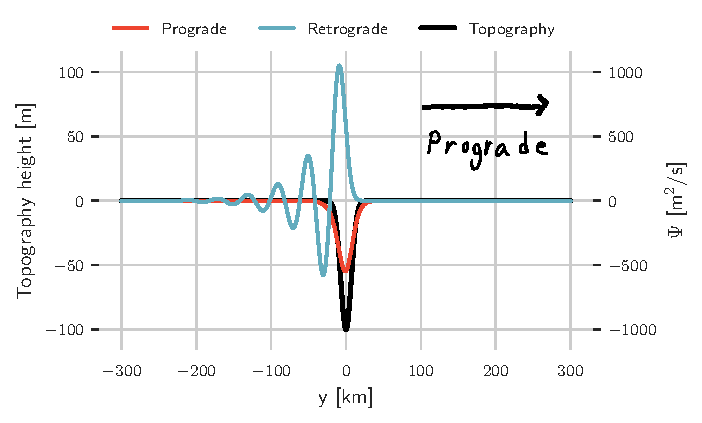
\includegraphics[width=\textwidth]{figures/psi_pro.pdf}
\end{figure}}

\only<3>{
\begin{figure}
\centering
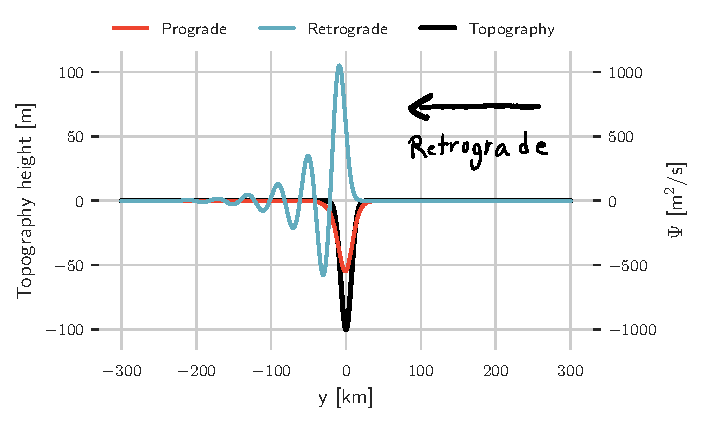
\includegraphics[width=\textwidth]{figures/psi_retro.pdf}
\end{figure}}

\end{frame}

%\begin{frame}{Theoretical response}
%\begin{columns}[t]
%\column{0.5\textwidth}
%\textbf{Retrograde}
%\begin{itemize}
%    \item Resonance can occur between the topography and the arrested wave.
%    \item The resonant streamfunction is 90\textdegree out of phase with the topography.
%\end{itemize}
%Quantitatively test this by comparing the wavelength of the lee wave with the wavelength of the arrested wave.

%\column{0.5\textwidth}
%\textbf{Prograde}
%\begin{itemize}
%    \item The streamlines resembles the topography, acting as a long-pass filter.
%    \item As the corresponding arrested wavenumber decreases, the flow becomes smoother.
%\end{itemize}
%Qualitatively test this by checking if decreasing arrested wavenumber gives a smoother flow. 

%\end{columns}
%\end{frame}

\section{Numerical experiments}
\begin{frame}
\frametitle{Model bathymetry used in ROMS}

\only<1>{
\begin{figure}
\centering
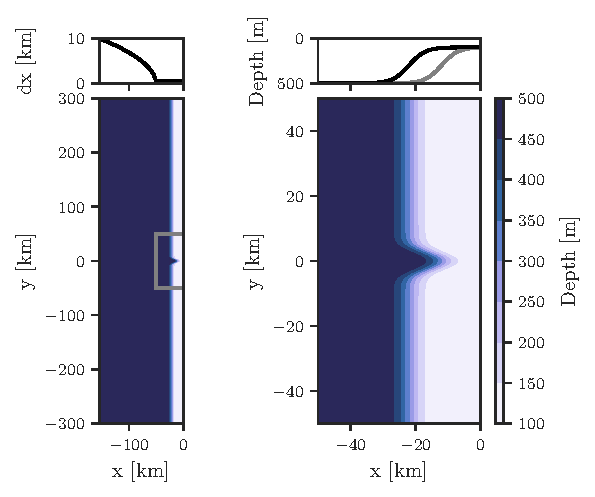
\includegraphics[clip, trim=0 0 0 0.3cm, width=0.8\textwidth]{figures/bathymetry.pdf}
\end{figure}}

\only<2>{
\begin{figure}
\centering
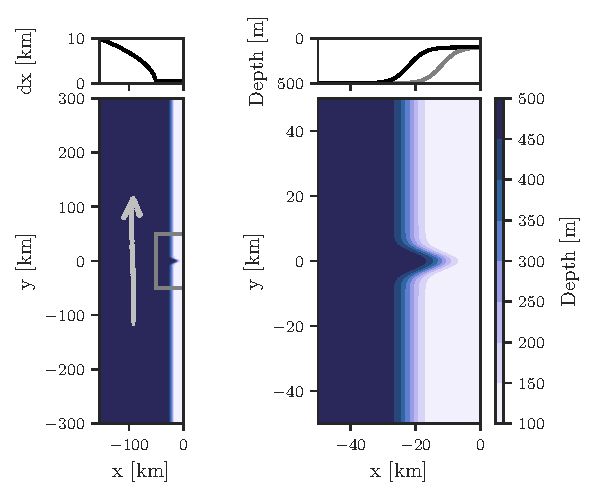
\includegraphics[clip, trim=0 0 0 0.3cm, width=0.8\textwidth]{figures/bathymetry_prograde.pdf}
\end{figure}}

\only<3>{
\begin{figure}
\centering
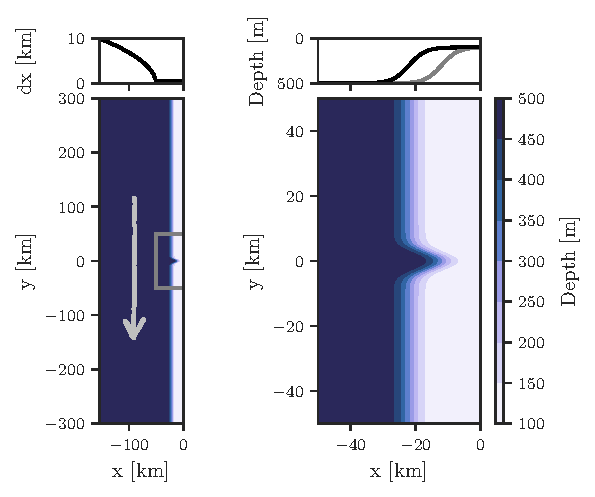
\includegraphics[clip, trim=0 0 0 0.3cm, width=0.8\textwidth]{figures/bathymetry_retrograde.pdf}
\end{figure}}

\end{frame}

%\begin{frame}
%\frametitle{Tracer distribution and model levels}
%\begin{figure}
%\centering
%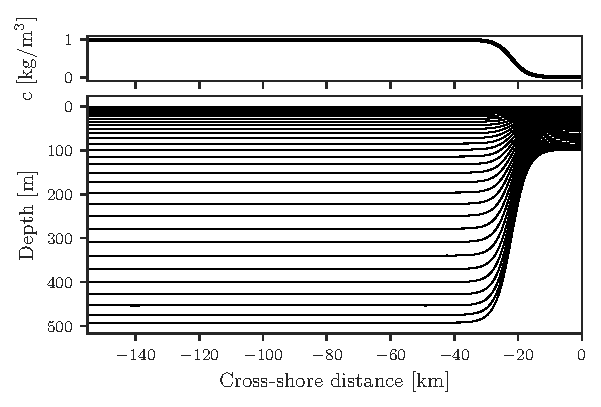
\includegraphics{figures/s-levels_tracers.pdf}
%\end{figure}
%\end{frame}

%\begin{frame}
%\frametitle{Forcing}
%\begin{figure}
%\centering
%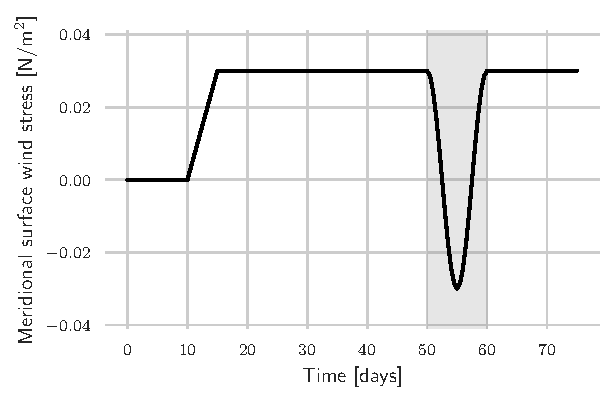
\includegraphics{figures/forcing.pdf}
%\end{figure}
%\end{frame}

\section{Results}

\subsection{General flow pattern}

\begin{frame}{Mean streamlines between day 40 and 50 at 95m depth}
%\begin{figure}
%\centering
%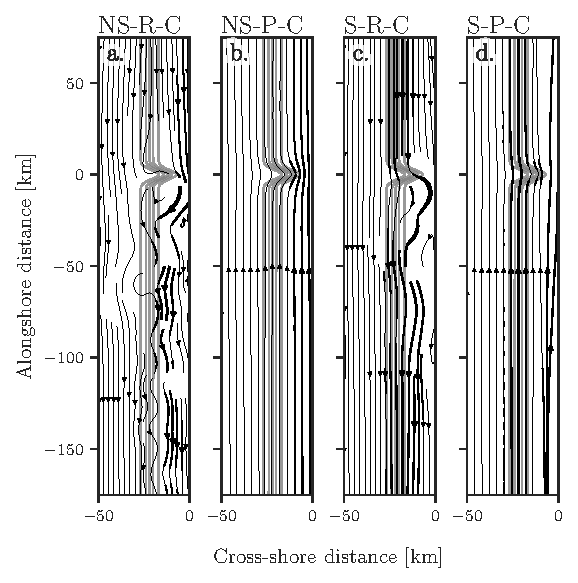
\includegraphics[width=0.7\textwidth]{figures/mean_streamlines_canyon_z95_40-50.pdf}
%\end{figure}
\only<1>{
\begin{figure}
\centering
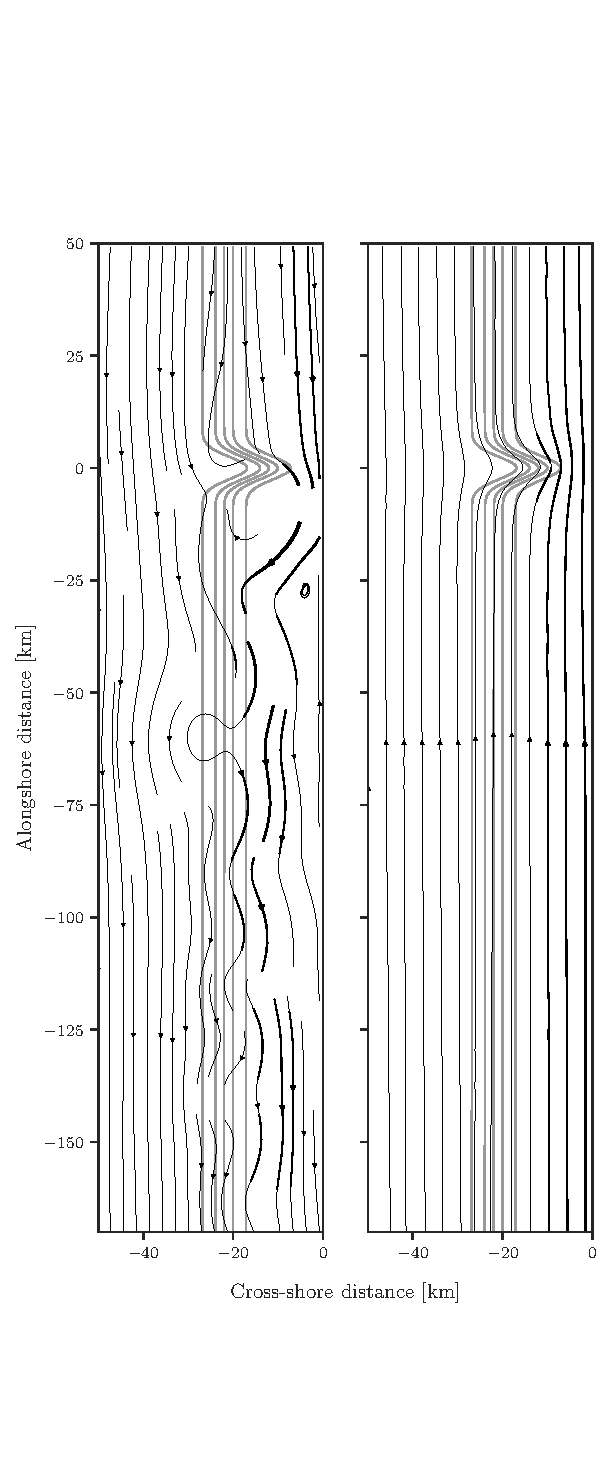
\includegraphics[clip, trim=0 0 0 3cm, width=0.37\linewidth]{figures/streamlines1.pdf}
\end{figure}}

\only<2>{
\begin{figure}
\centering
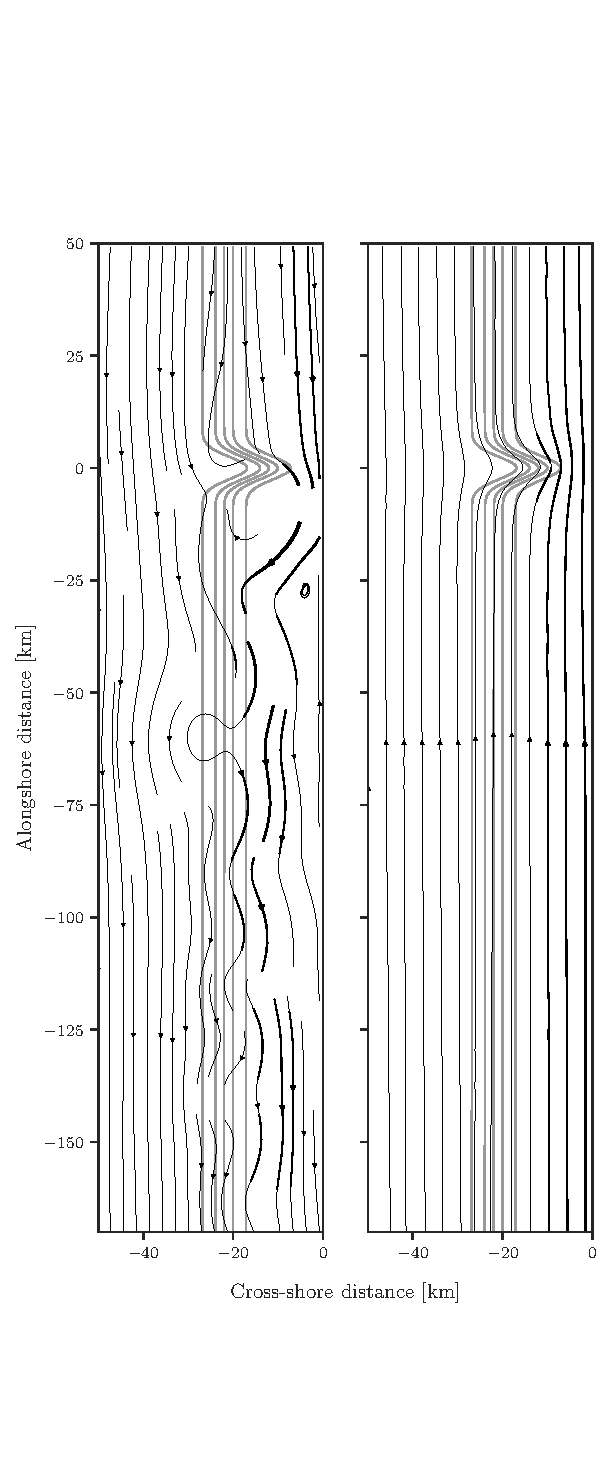
\includegraphics[clip, trim=0 0 0 3cm, width=0.37\linewidth]{figures/streamlines1.pdf}
\end{figure}}

\only<3>{
\begin{figure}
\centering
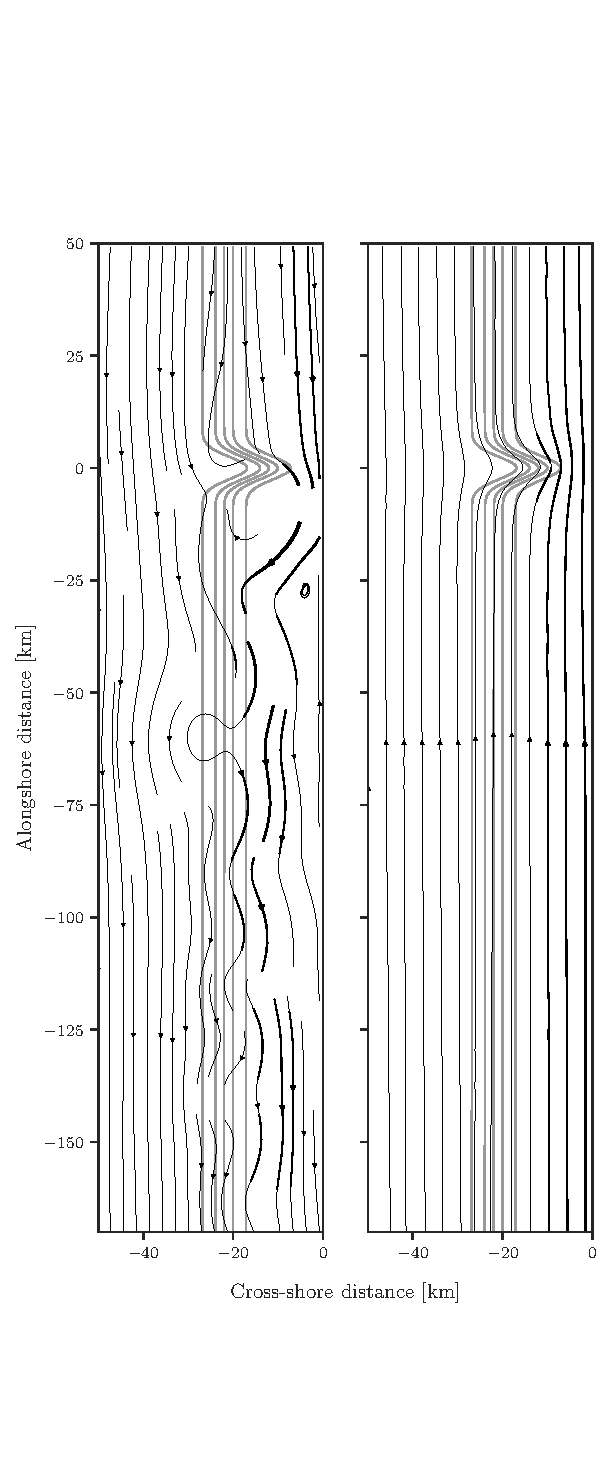
\includegraphics[clip, trim=0 0 0 3cm, width=0.37\linewidth]{figures/streamlines1.pdf}
\end{figure}}

\end{frame}

%\begin{frame}{Hovmöller diagrams of SSH anomalies, unstratified system}
%\begin{figure}
%\centering
%\includegraphics{figures/Unstratified_zeta_hovmoller.pdf}
%\end{figure}
%\end{frame}

%\begin{frame}{Hovmöller diagrams of SSH anomalies, stratified system}
%\begin{figure}
%\centering
%\includegraphics{figures/Stratified_zeta_hovmoller.pdf}
%\end{figure}
%\end{frame}

\subsection{Comparison with QG theory}

\begin{frame}{Analytical vs. modeled arrested wavelength}
\begin{figure}
\centering
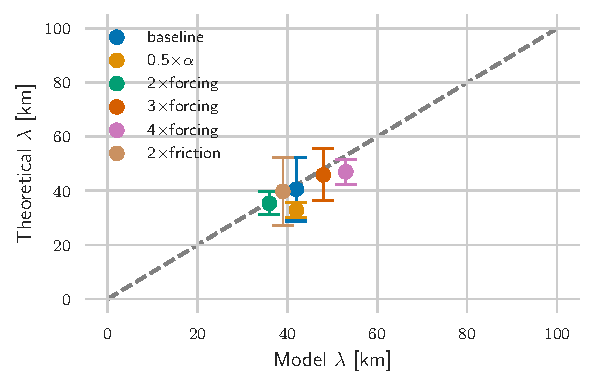
\includegraphics{figures/Unstratified_theoreticalVSmodel_wave_length.pdf}
\end{figure}
\end{frame}

%\begin{frame}{Stratified system: theoretical vs. modeled arrested wavelength}
%\begin{figure}
%\centering
%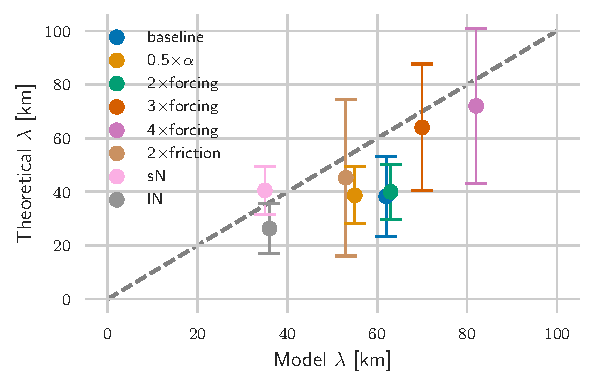
\includegraphics{figures/Stratified_theoreticalVSmodel_wave_length_xzshear.pdf}
%\end{figure}
%
%\begin{frame}{Streamlines for prograde flow in an unstratified system}
%\begin{figure}
%\centering
%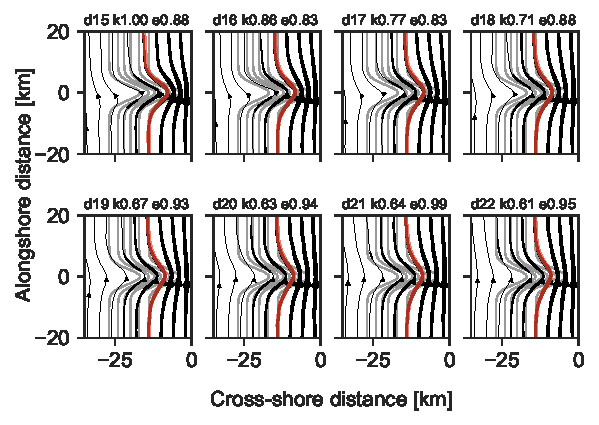
\includegraphics{figures/streamlines_Unstratified_z95_from_south_canyon_period1_k.pdf}
%\end{figure}
%\end{frame}

%\begin{frame}{Streamlines for prograde flow in a stratified system}
%\begin{figure}
%\centering
%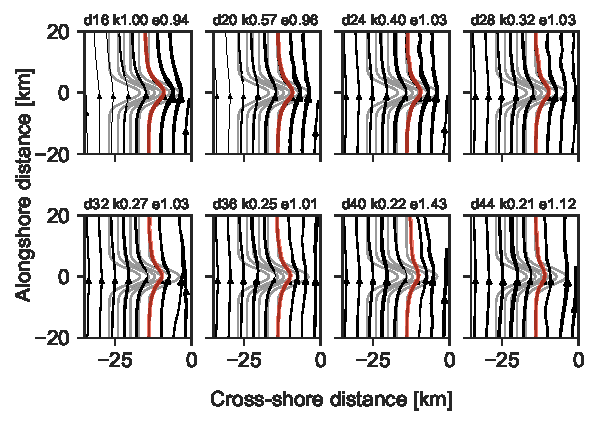
\includegraphics{figures/streamlines_Stratified_z95_from_south_canyon_period1_k.pdf}
%\end{figure}
%\end{frame}

\subsection{Cross-slope tracer transport}

\begin{frame}
\frametitle{Model bathymetry $\varpropto$ tracer distribution}
\begin{figure}
\centering
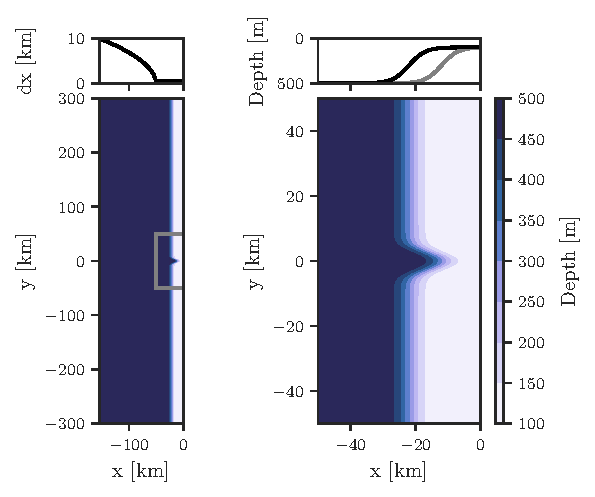
\includegraphics[clip, trim=0 0 0 0.3cm, width=0.8\textwidth]{figures/bathymetry.pdf}
\end{figure}
\end{frame}

%\begin{frame}{Early stages: cumulative tracer transport, model run - no model run}
%\begin{figure}
%\centering
%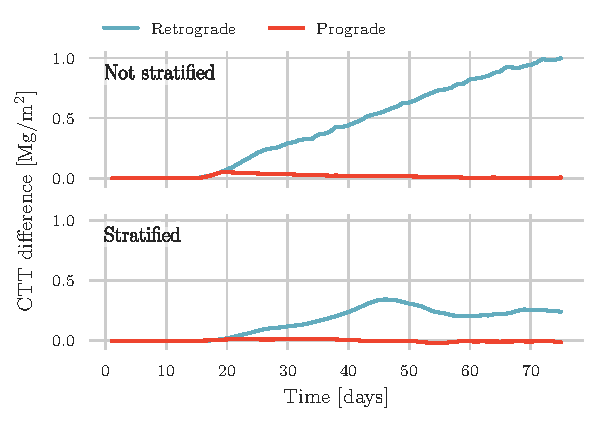
\includegraphics{figures/Huon_dye_01_cumulative_transport_diff_baseline.pdf}
%\end{figure}
%\end{frame}

\begin{frame}{Evolution of eddy kinetic energy}

\only<1>{
\begin{figure}
\centering
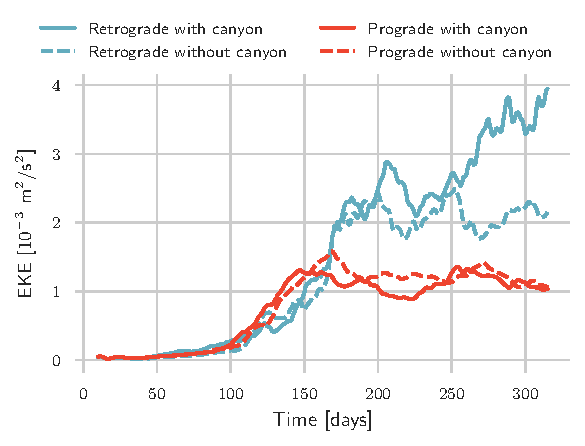
\includegraphics{figures/EKE_MKE_temporal_mean_Stratified.pdf}
\end{figure}}


\only<2>{
\begin{figure}
\centering
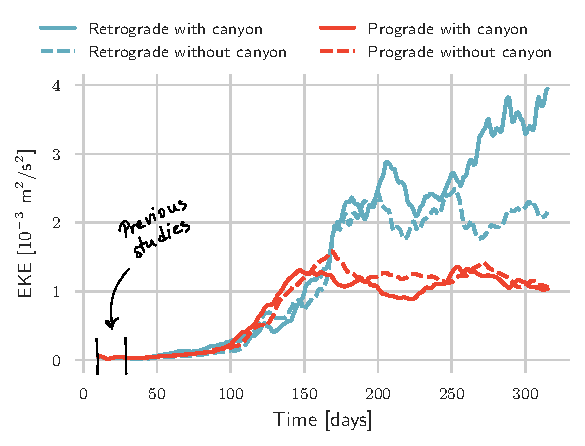
\includegraphics{figures/EKE2.pdf}
\end{figure}}


\only<3>{
\begin{figure}
\centering
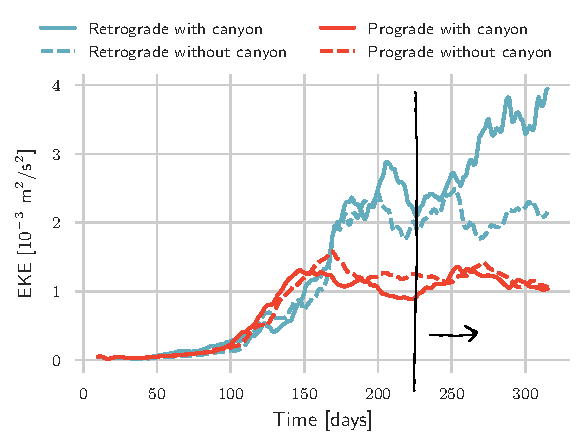
\includegraphics{figures/EKE3.pdf}
\end{figure}}
\end{frame}

%\begin{frame}{Early stages: cumulative tracer transport}
%\begin{figure}
%\centering
%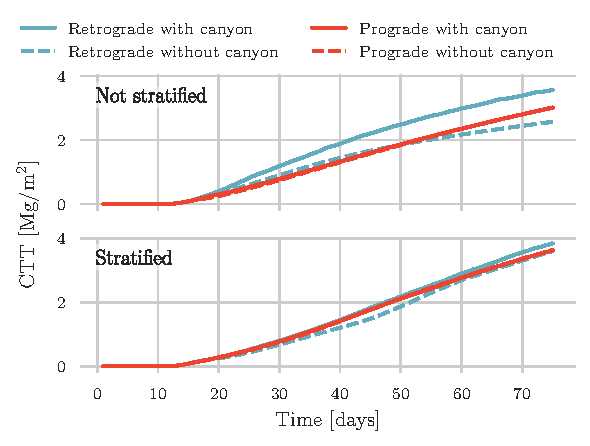
\includegraphics{figures/Huon_dye_01_cumulative_transport_baseline.pdf}
%\end{figure}
%\end{frame}

\begin{frame}{Turbulent stages: retrograde tracer transport}
\begin{figure}
\centering
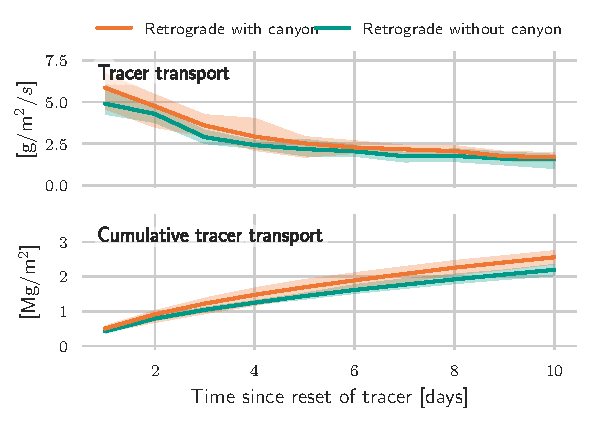
\includegraphics{figures/exchange_Retrograde_composite_Stratified.pdf}
\end{figure}
\end{frame}

\begin{frame}{Turbulent stages: prograde tracer transport}
\begin{figure}
\centering
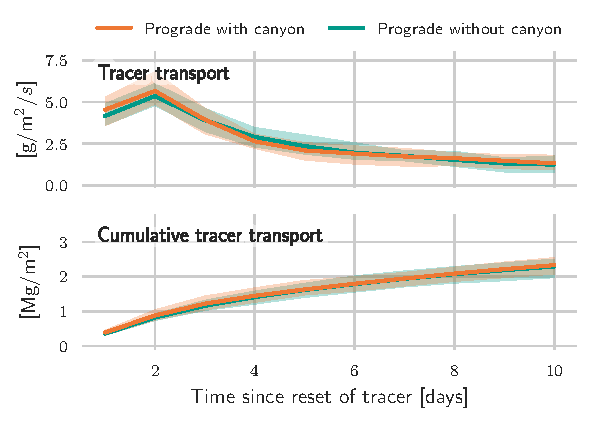
\includegraphics{figures/exchange_Prograde_composite_Stratified.pdf}
\end{figure}
\end{frame}

\begin{frame}{Wind event: prograde tracer transport}
\begin{figure}
\centering
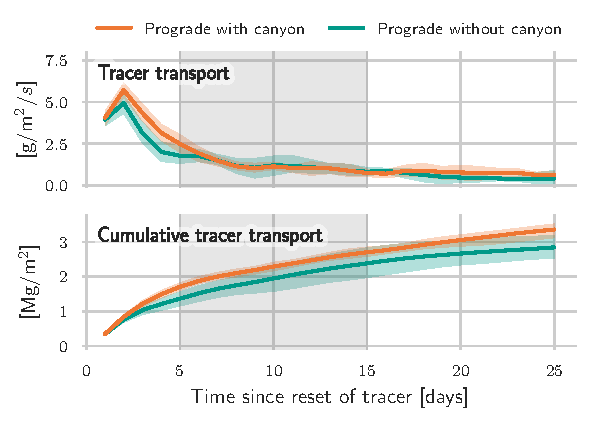
\includegraphics{figures/exchange_Prograde_composite_Event.pdf}
\end{figure}
\end{frame}

\begin{frame}{Wind event: bottom velocity and EKE}
\begin{figure}
\centering
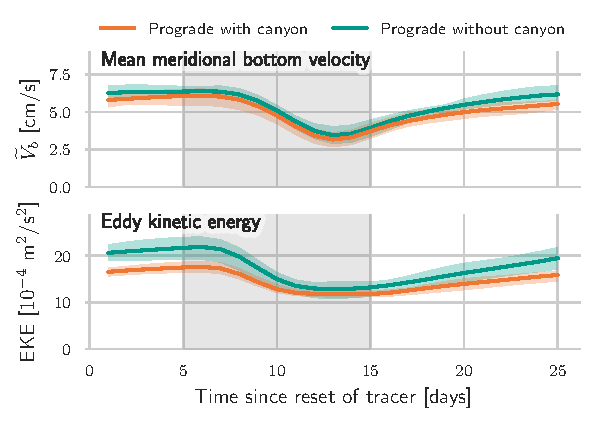
\includegraphics{figures/v_eke_Prograde_composite_Event.pdf}
\end{figure}
\end{frame}

%\section{Applicability to LoVe}

%\subsection{Applicability to LoVe}
%\begin{frame}{Applicability to LoVe}
%\begin{itemize}
%    \item There are episodically reversal of winds in LoVe
%    \item Role of multiple succeeding canyons 
%\end{itemize}

%\begin{figure}
%\centering
%\includegraphics[width=0.5\textwidth]{figures/dybdedata_lite.pdf}
%\end{figure}

%\end{frame}

\section{Conclusion}
\begin{frame}{Conclusion}
\begin{itemize}
    \item There is generally good agreement between analytical, quasi-geostrophic models and numerical model runs.
    \item A canyon enhances the cross-slope tracer transport under retrograde flow conditions, also in a highly turbulent field.
    \item With the presence of periods of reversed winds, a canyon enhanced the transport, also under prograde conditions.
\end{itemize} 
\end{frame}





\begin{frame}
\frametitle{References}
\footnotesize{
\begin{thebibliography}{99} % Beamer does not support BibTeX so references must be inserted manually as below
\bibitem[Christensen, 1992]{p1} Christensen, Ivar and Haug, Tore and Øien, Nils (1992)
\newblock Seasonal distribution, exploitation and present abundance of stocks of large baleen whales (Mysticeti) and sperm whales (Physeter macrocephalus) in Norwegian and adjacent waters
\newblock \emph{ICES journal of marine science} 49(3), 341--355.

\bibitem[Zhang and Lentz, 2017]{p2} Zhang, Weifeng  and Lentz, Steven J (2017)
\newblock Wind-Driven Circulation in a Shelf Valley. Part I: Mechanism of the Asymmetrical Response to Along-Shelf Winds in Opposite Directions
\newblock \emph{Journal of physical oceanography} 47(12), 2927--2947.
\end{thebibliography}
}
\end{frame}

%------------------------------------------------

\begin{frame}
\Huge{Thank you for your attention!}
%\Huge{\centerline{The End}}
\begin{figure}
\centering
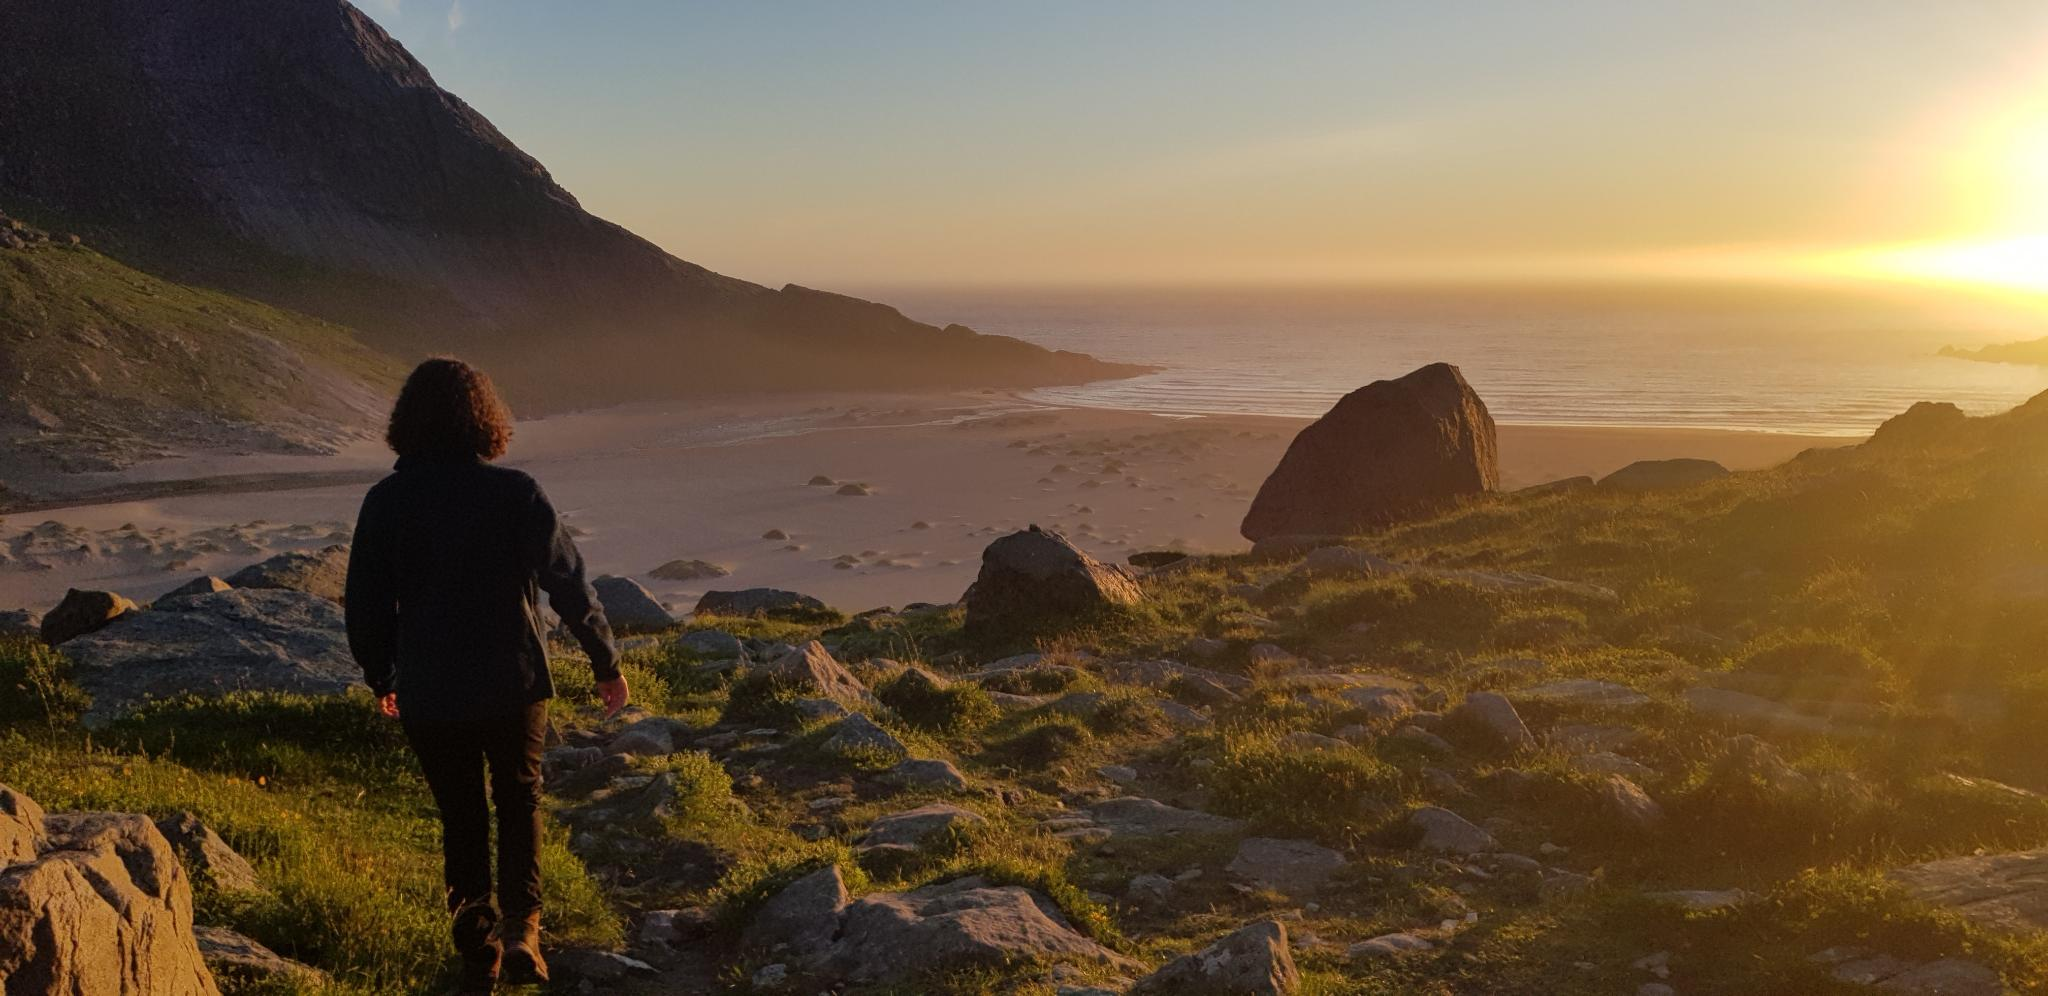
\includegraphics[width=\textwidth]{figures/meg.jpeg}
\end{figure}
\end{frame}

%----------------------------------------------------------------------------------------
%   SUPPLEMENTARY SLIDES
%----------------------------------------------------------------------------------------
%\appendix

%\begin{frame}{Supplementary figure}
%This slide is not part of total slide count or the navigational panel.
%\begin{figure}
%    \centering
%    \missingfigure{Insert supplementary figure here.}
%\end{figure}
%\end{frame}

%----------------------------------------------------------------------------------------

\end{document} 